%Template desenvolvido por Jorge Luiz Ferreira da Silva Junior
%Contato: jorgeluizjk@gmail.com
%Repositório disponível em: https://github.com/Collumbus/Template_Slides_LaTex
%Criado em 18 de julhor de 2018.

\documentclass[aspectratio=169]{beamer}
\usetheme{default} %tema do slide
\usecolortheme{seagull}
\usepackage[brazil]{babel} %texto
\usepackage[utf8]{inputenc} %texto
\usepackage{graphicx} %imagem	
\usepackage{caption} %imagem
\usepackage{subcaption} %imagem
\usepackage{float} %imagem e tabelas
\usepackage{booktabs} %tabelas	
\usepackage[abnt-emphasize=bf,alf]{abntex2cite} %citacoes ABNT
\graphicspath{{./Figuras/}} %Colarimages na pasta "Figuras". Gosto de fazer isso para organizar os arquivos.    		

%Plano de fundo: Barra verde
\setbeamertemplate{background canvas}{
\includegraphics
	[width=\paperwidth,height=\paperheight]{bkg.jpg}}
	
%Caso queira mudar a paleta de cores editar os parâmetros abaixo	
%\definecolor{mygreen}{rgb}{.125,.5,.25}
%\usecolortheme[named=mygreen]{structure}


\usepackage{textpos}

%Logo da UnB
\addtobeamertemplate{headline}{}{%
\begin{textblock*}{100mm}(.030\textwidth,0.2cm)

\includegraphics[width=1cm]{logo2}
\end{textblock*}}

%Logo do Mestrado
\addtobeamertemplate{headline}{}{%
\begin{textblock*}{100mm}(.110\textwidth,0.17cm)

\includegraphics[width=1cm]{logo4}
\end{textblock*}}

%Logo da FGA
\addtobeamertemplate{headline}{}{%
\begin{textblock*}{100mm}(.915\textwidth,0.1cm)

\includegraphics[width=1.0cm]{logo3} 
\end{textblock*}}


\begin{document}
	%Título
	\title[Título Curto]{Título longo}
	%Funções desativadas neste template
	%\author[jorgeluizjk@gmail.com]{Jorge Luiz Ferreira da Silva Junior}
	%\institute[]{UnB}
	\date[]{}%Não mexer nesta função
	
	\setbeamertemplate{frametitle}[default][center]
	
	\begin{frame}
	
		%Cabeçalho
		\frametitle{\tiny  \textbf{Universidade de Brasília – UnB\\Faculdade UnB Gama – FGA\\ \vspace{0.8mm} Mestrado em Engenharia Biomédica\\ \qquad}}
		\titlepage
		
		%Autor / Orientador
		\begin{textblock*}{100mm}(.35\textwidth,-2.5cm)
			\begin{flushright}
				\footnotesize
				Autor: Nome do Autor\\
				Orientadora: Nome do Orientador(a)\\
				Coorientadora: Nome do Coorientador(a)
			\end{flushright}
		\end{textblock*}

		%Data
		\begin{textblock*}{50mm}(.3\textwidth,-0.5cm)
			\begin{center}
				\footnotesize
				Brasília, 09 de Agosto de 2018\\
				UnB/FGA
			\end{center}
		\end{textblock*}

	\end{frame}
	
	\begin{frame}
		\frametitle{Sum\'{a}rio}
		\tableofcontents%[pausesections]
	\end{frame}
	
%---------------------------------------------------------------------------
	% PRIMEIRA SECAO
	\section{Imagem}
%---------------------------------------------------------------------------

	% SLIDE 1 - APENAS UMA IMAGEM	
	\begin{frame}
		\frametitle{Imagem}
		\framesubtitle{Imagens simples}
		Imagine a Figura:
		
		\begin{figure}
			\centering
			\caption{Legenda da figura}
			
			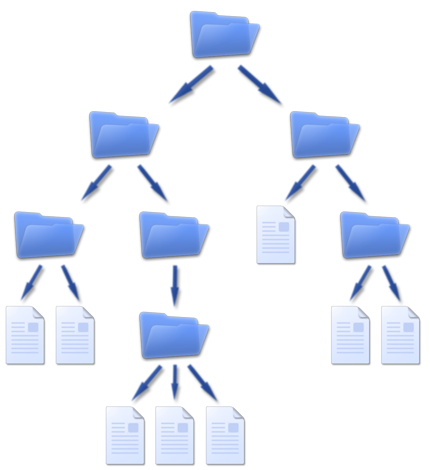
\includegraphics[width=.25\linewidth]{sa.png} 
			
			\footnotesize{Fonte: ...	
				\par Visitado em \today.}
			\label{im1}
		\end{figure}	
	\end{frame}
	
	% SLIDE 2 - APENAS UMA IMAGEM	
	\begin{frame}
		\frametitle{Imagem}
		\framesubtitle{Imagens simples sem legenda}
			Imagine a Figura:
		
			\center
			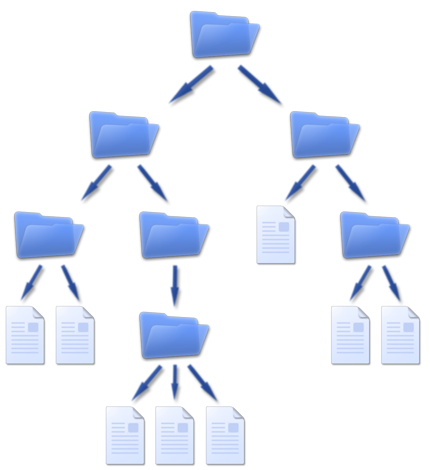
\includegraphics[width=.25\linewidth]{sa.png} 	
	\end{frame}
	
	% SLIDE 3 - TEXTO SEGUIDO DE UMA IMAGEM	
	\begin{frame}
		\frametitle{Imagem}
		\framesubtitle{Imagens agrupadas}
		Imagine a Figura:
		
		\begin{figure}[H]
			\centering
			\caption{Legenda da figura}
			\begin{subfigure}{0.45\textwidth}
				\centering
				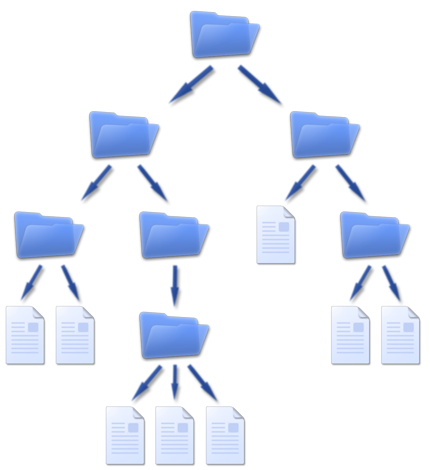
\includegraphics[width=.25\linewidth]{sa.png}
				\caption{Legenda da parte 1}
				\label{figPt1}
			\end{subfigure}
			\hfill
			\begin{subfigure}{0.45\textwidth}
				\centering
				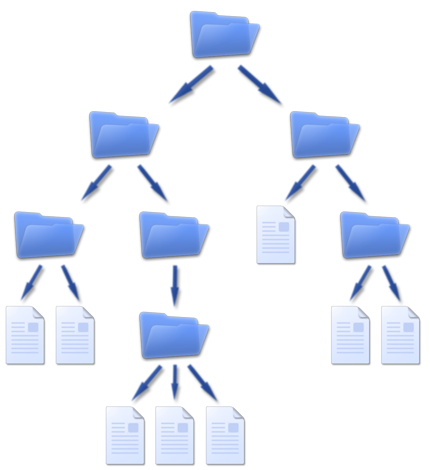
\includegraphics[width=.25\linewidth]{sa.png}
				\caption{Legenda da parte 2}
				\label{figPt2}
			\end{subfigure}                                                   
			
			\footnotesize{Fonte: \citeonline{tanebaun2010}}
			\label{figPt1e2}
		\end{figure}	
	\end{frame}
	
	% SLIDE 4 - TEXTO EM UMA COLUNA, IMAGEM EM OUTRA COLUNA	
	\begin{frame}
		\frametitle{Imagem}
		\framesubtitle{Imagem e texto}
		
		\begin{minipage}[H]{.5\textwidth}
			Texto texto texto texto texto texto texto texto texto texto texto texto texto texto texto texto texto texto texto texto texto texto texto texto texto texto texto texto texto texto texto texto texto texto texto texto texto texto texto texto texto texto texto texto texto texto texto texto texto texto texto texto texto texto texto texto texto texto texto texto texto texto texto texto texto texto texto texto texto texto texto texto texto texto texto texto texto texto texto texto texto texto texto texto texto texto texto.	
		\end{minipage}
		\hfill
		\begin{minipage}[H]{.45\textwidth}
			\begin{figure}
				\centering
				\caption{Legenda da imagem}
				
				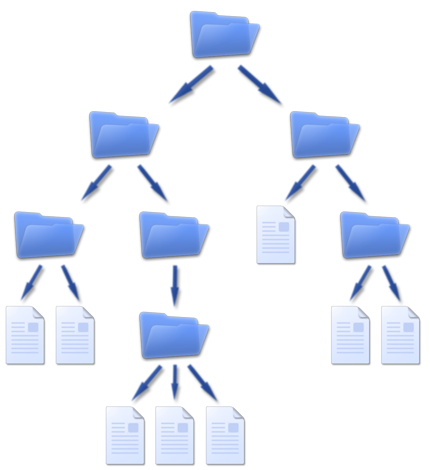
\includegraphics[width=.25\linewidth]{sa.png}
				
				\footnotesize{Fonte: \citeonline{tanebaun2010}}
				\label{figtextimg}
			\end{figure}  
		\end{minipage}
	\end{frame}
	
%---------------------------------------------------------------------------
	% SEGUNDA SECAO
	\section{Tabelas}	
%---------------------------------------------------------------------------
	% SLIDE 5 - UMA TABELA	
	\begin{frame}
		\frametitle{Tabelas}
				
		\begin{table}[H]
			\centering
			\caption{Atributos dos arquivos}
			\begin{tabular}{c|c}
				\toprule
				\textbf{Atributo} & \textbf{Significado} \\
				\midrule
				Prote\c{c}\~{a}o&Quem tem acesso ao arquivo e de que modo\\
				\midrule
				Senha&Necessidade de senha para acesso ao arquivo\\
				\midrule
				Criador&ID do criador do arquivo\\
				\midrule
				Propriet\'{a}rio&Propriet\'{a}rio atual\\
				\bottomrule
			\end{tabular}
			
			\label{tab:attI}
			\footnotesize{Fonte: \citeonline{tanebaun2010}}				
		\end{table}
	\end{frame}
	
%---------------------------------------------------------------------------
	% TERCEIRA SECAO
	\section{Listas}
%---------------------------------------------------------------------------
	% SLIDE 6 - LISTAGEM SIMPLES
	\begin{frame}
		\frametitle{Listas}
		\framesubtitle{Listas Simples}
		\begin{itemize}
			\item \textit{Create};
			\item \textit{Delete};
			\item \textit{Open};
			\item \textit{Close};
			\item \textit{Read};
		\end{itemize}
	\end{frame}
	
	% SLIDE 7 - LISTAS E SUBLISTAS
	\begin{frame}
		\frametitle{Listas}
		\framesubtitle{Listas e sublistas}
		\begin{itemize}
			\item \textit{Create};
			\begin{itemize}
				\item \textit{Open};
				\item \textit{Close};
				\item \textit{Read};
			\end{itemize}
			\item \textit{Delete};
			
		\end{itemize}
	\end{frame}
	
%---------------------------------------------------------------------------
	%SECAO DE REFERENCIAS
	\section{Refer\^{e}ncias bibliogr\'{a}ficas}
%---------------------------------------------------------------------------
	% SLIDE 8 - REFERENCIAS
	\begin{frame}
		\frametitle{Refer\^{e}ncias bibliogr\'{a}ficas indiretas}
		\textbackslash citeonline\{labelDaReferencia\}\\
		\textbf{Resultado}: De acordo com \citeonline{tanebaun2010}, os computadores...
	\end{frame}
		
	% SLIDE 9 - REFERENCIAS
	\begin{frame}
		\frametitle{Refer\^{e}ncias bibliogr\'{a}ficas diretas}
		\textbackslash cite[p. \~{}45]\{labelDaReferencia\} \\
		\textbf{Resultado}: "os computadores..." \cite[p.~45]{tanebaun2010} 
	\end{frame}	

	% SLIDE 10 - REFERENCIAS
	\begin{frame}
		%[allowframebreaks]
		\frametitle{Refer\^{e}ncias bibliogr\'{a}ficas}
		\bibliography{Referencias}
	\end{frame}
	%---------------------------------------------------------------------------
\end{document}
